\documentclass[aspectratio=169,10pt]{beamer}

\usepackage[default]{sourcesanspro}
\usepackage{fontawesome5}
\usepackage{booktabs}
\usepackage{tabularx}
\usepackage{array}
\usepackage{tikz}
\usetikzlibrary{arrows.meta,positioning,shapes.geometric,calc,backgrounds}
\usepackage{graphicx}
\usepackage[backend=biber,style=numeric,sorting=none]{biblatex}
\addbibresource{references.bib}

\definecolor{Navy}{HTML}{17324D}
\definecolor{Blue}{HTML}{247BA0}
\definecolor{Teal}{HTML}{20A39E}
\definecolor{Amber}{HTML}{E09F3E}
\definecolor{Red}{HTML}{C94C4C}
\definecolor{Ink}{HTML}{243447}
\definecolor{Muted}{HTML}{64748B}
\definecolor{Mist}{HTML}{E8EEF2}
\definecolor{Wash}{HTML}{F5F8FA}
\definecolor{PaleTeal}{HTML}{E7F7F5}
\definecolor{PaleAmber}{HTML}{FFF4E3}
\definecolor{PaleRed}{HTML}{FCECEC}

\setbeamercolor{normal text}{fg=Ink,bg=white}
\setbeamercolor{frametitle}{fg=Navy,bg=white}
\setbeamercolor{structure}{fg=Teal}
\setbeamerfont{frametitle}{size=\Large,series=\bfseries}
\setbeamertemplate{navigation symbols}{}
\setbeamertemplate{itemize item}{\color{Teal}\raise0.2ex\hbox{\tiny\faCircle}}
\setbeamersize{text margin left=0.55cm,text margin right=0.55cm}

\setbeamertemplate{frametitle}{%
  \vspace{0.20cm}\insertframetitle\par
  \vspace{-0.12cm}\color{Teal}\rule{1.05cm}{1.5pt}\color{Mist}\rule{\dimexpr\textwidth-1.05cm\relax}{1.5pt}
}
\setbeamertemplate{footline}{%
  \leavevmode\hbox{%
    \begin{beamercolorbox}[wd=.78\paperwidth,ht=2.7ex,dp=1.1ex,leftskip=.55cm]{normal text}%
      \color{Muted}\scriptsize FOR2107 × Tozzi · preliminary · 23 July 2026
    \end{beamercolorbox}%
    \begin{beamercolorbox}[wd=.22\paperwidth,ht=2.7ex,dp=1.1ex,rightskip=.55cm plus1fil]{normal text}%
      \color{Muted}\scriptsize\insertframenumber/6
    \end{beamercolorbox}%
  }
}

\newcommand{\kpi}[2]{%
  \begin{minipage}[c][0.73cm][c]{0.17\textwidth}\centering
    {\color{Navy}\fontsize{20}{20}\selectfont\bfseries #1}\\[-1pt]
    {\color{Muted}\scriptsize\MakeUppercase{#2}}
  \end{minipage}}
\newcommand{\statusline}[3]{%
  \par\vspace{0.10cm}\noindent{\color{#1}#2}\hspace{0.13cm}{\scriptsize #3}\par}
\newcommand{\matchmark}{\color{Teal}\faCheckCircle}
\newcommand{\partialmark}{\color{Amber}\faExclamationCircle}
\newcommand{\missingmark}{\color{Red}\faTimesCircle}
\newcommand{\pendingmark}{\color{Muted}\faMinusCircle}

\begin{document}

% ---------------------------------------------------------------------------
\setbeamertemplate{background}{\includegraphics[width=\paperwidth,height=\paperheight]{figures/circuit_landscape.png}}
\setbeamertemplate{footline}{}
\begin{frame}[plain]
  \begin{tikzpicture}[remember picture,overlay]
    \fill[Navy,opacity=.18] (current page.south west) rectangle (current page.north east);
    \node[anchor=west,text width=7.35cm] at ([xshift=.75cm,yshift=.45cm]current page.west) {%
      {\color{Teal}\small\bfseries PRELIMINARY RESULTS \;·\; SCIENTIFIC ADVISORY UPDATE}\par
      \vspace{0.22cm}
      {\color{white}\fontsize{29}{31}\selectfont\bfseries Resting-state circuit profiles are operational}\par
      \vspace{0.18cm}
      {\color{white!76}\large FOR2107 adaptation of Tozzi et al. (2024)}\par
      \vspace{0.48cm}
      {\color{white!70}\small 75 scans \;·\; 67 selected \;·\; 3 rest-FC features}\par
      \vspace{0.62cm}
      {\color{white!62}\scriptsize 23 July 2026 \hspace{0.35cm} | \hspace{0.35cm} Decision focus: what is demonstrated—and what is not}
    };
  \end{tikzpicture}
\end{frame}
\setbeamertemplate{background}{}
\setbeamertemplate{footline}{%
  \leavevmode\hbox{%
    \begin{beamercolorbox}[wd=.78\paperwidth,ht=2.7ex,dp=1.1ex,leftskip=.55cm]{normal text}\color{Muted}\scriptsize FOR2107 × Tozzi · preliminary · 23 July 2026\end{beamercolorbox}%
    \begin{beamercolorbox}[wd=.22\paperwidth,ht=2.7ex,dp=1.1ex,rightskip=.55cm plus1fil]{normal text}\color{Muted}\scriptsize\insertframenumber/6\end{beamercolorbox}%
  }}

% ---------------------------------------------------------------------------
\begin{frame}{Tozzi in one frame}
\centering
\begin{tikzpicture}[
  node distance=0.28cm,
  box/.style={rounded corners=3pt,minimum height=1.25cm,text width=2.05cm,align=center,fill=Wash,draw=Mist,line width=.7pt,font=\scriptsize},
  arrow/.style={-{Stealth[length=2.2mm]},line width=1.0pt,color=Teal}
]
  \node[box] (input) {\color{Blue}\faBrain\\[-1pt]\textbf{Rest + tasks}\\{\tiny D/S/A · faces · Go/NoGo}};
  \node[box,right=of input] (roi) {\color{Teal}\faProjectDiagram\\[-1pt]\textbf{41 regional}\\{\tiny circuit scores}};
  \node[box,right=of roi] (norm) {\color{Amber}\faBalanceScale\\[-1pt]\textbf{Healthy norm}\\{\tiny participant-level SD}};
  \node[box,right=of norm] (dist) {\color{Blue}\faGripHorizontal\\[-1pt]\textbf{Geometry}\\{\tiny $d_{ij}=1-r_{ij}$}};
  \node[box,right=of dist] (cluster) {\color{Teal}\faSitemap\\[-1pt]\textbf{Average linkage}\\{\tiny candidate biotypes}};
  \node[box,right=of cluster] (valid) {\color{Amber}\faCheckDouble\\[-1pt]\textbf{Convergence}\\{\tiny stability · nulls · clinical}};
  \draw[arrow] (input)--(roi); \draw[arrow] (roi)--(norm); \draw[arrow] (norm)--(dist);
  \draw[arrow] (dist)--(cluster); \draw[arrow] (cluster)--(valid);
\end{tikzpicture}

\vspace{0.28cm}
\begin{columns}[T,onlytextwidth]
  \begin{column}{0.36\textwidth}
    \begin{beamercolorbox}[rounded=true,sep=.22cm]{block body}
      {\color{Navy}\small\bfseries Scientific objective}\par\vspace{.08cm}
      \scriptsize Replace diagnostic averages with interpretable, individual circuit-dysfunction profiles—and test whether profile-defined groups differ clinically.
    \end{beamercolorbox}
    \vspace{.18cm}
    {\color{Muted}\tiny Task conditions contribute condition-specific activation/connectivity scores; task-free connectivity is quantified independently.}
  \end{column}
  \begin{column}{0.29\textwidth}
    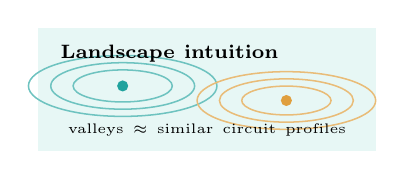
\begin{tikzpicture}[x=0.63cm,y=0.37cm]
      \fill[PaleTeal] (0,0) rectangle (6.8,4.25);
      \foreach \s/\c in {1.0/Teal,1.45/Teal,1.9/Teal}{\draw[\c!65,line width=.55pt] (1.7,2.25) ellipse ({\s} and {0.55*\s});}
      \foreach \s/\c in {.9/Amber,1.35/Amber,1.8/Amber}{\draw[\c!70,line width=.55pt] (5.0,1.75) ellipse ({\s} and {0.55*\s});}
      \fill[Teal] (1.7,2.25) circle (2pt); \fill[Amber] (5.0,1.75) circle (2pt);
      \node[anchor=north west,text width=3.9cm] at (.25,4.0) {\scriptsize\bfseries Landscape intuition};
      \node[anchor=south,text width=3.8cm,align=center] at (3.4,.18) {\tiny valleys $\approx$ similar circuit profiles};
    \end{tikzpicture}
  \end{column}
  \begin{column}{0.31\textwidth}
    \begin{beamercolorbox}[rounded=true,sep=.22cm]{block body}
      {\color{Red}\scriptsize\bfseries Important distinction}\par\vspace{.08cm}
      \scriptsize Tozzi does \textbf{not} fit an explicit energy function. “Landscape” is only an intuition for basins in correlation-distance feature space.
    \end{beamercolorbox}
    \vspace{.20cm}
    {\color{Muted}\tiny Source: Tozzi et al., \textit{Nature Medicine} 2024\,\cite{tozzi2024}. Diagram recreated; no publication figure copied.}
  \end{column}
\end{columns}
\end{frame}

% ---------------------------------------------------------------------------
\begin{frame}{Current implementation status}
\begin{columns}[T,onlytextwidth]
  \begin{column}{0.322\textwidth}
    \begin{beamercolorbox}[rounded=true,sep=.22cm]{block body}
      {\color{Teal}\bfseries\faCheckCircle\hspace{.12cm} Implemented}\par\vspace{.05cm}
      \statusline{Teal}{\faCheck}{75 external MNI-2\,mm scans ingested}
      \statusline{Teal}{\faCheck}{Tozzi ROI extraction; Fisher-$z$ FC}
      \statusline{Teal}{\faCheck}{Healthy-reference standardization}
      \statusline{Teal}{\faCheck}{$1-r$ distance + average linkage}
      \statusline{Teal}{\faCheck}{Null/permutation, LOO, 80\%, split-half}
      \statusline{Teal}{\faCheck}{HTML/PDF report + 16 passing tests}
    \end{beamercolorbox}
  \end{column}
  \begin{column}{0.322\textwidth}
    \begin{beamercolorbox}[rounded=true,sep=.22cm]{block body}
      {\color{Amber}\bfseries\faExclamationCircle\hspace{.12cm} Partial}\par\vspace{.05cm}
      \statusline{Amber}{\faAdjust}{Preprocessing accepted, not reproduced}
      \statusline{Amber}{\faAdjust}{Provenance incomplete for cleaned scans}
      \statusline{Amber}{\faAdjust}{Motion QC unavailable; no FD exclusion}
      \statusline{Amber}{\faAdjust}{MDD/anxiety phenotype mapping operational}
      \statusline{Amber}{\faAdjust}{Validation runs = 50, not 10,000}
      \statusline{Amber}{\faAdjust}{Single site; small clinical sample}
    \end{beamercolorbox}
  \end{column}
  \begin{column}{0.322\textwidth}
    \begin{beamercolorbox}[rounded=true,sep=.22cm]{block body}
      {\color{Red}\bfseries\faTimesCircle\hspace{.12cm} Missing}\par\vspace{.05cm}
      \statusline{Red}{\faTimes}{Face-matching task contrasts + FC}
      \statusline{Red}{\faTimes}{Affective-priming contrasts + FC}
      \statusline{Red}{\faTimes}{Go/NoGo equivalent in FOR2107}
      \statusline{Red}{\faTimes}{Independent/leave-study-out validation}
      \statusline{Red}{\faTimes}{Treatment-response replication}
      \statusline{Red}{\faTimes}{Predeclared replication decision rule}
    \end{beamercolorbox}
  \end{column}
\end{columns}

\vspace{.28cm}
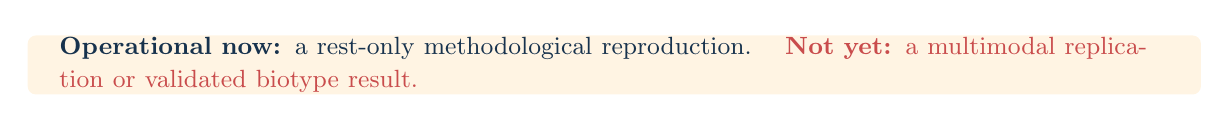
\begin{tikzpicture}
  \fill[PaleAmber,rounded corners=3pt] (0,0) rectangle (14.9,.75);
  \node[anchor=west,text width=14.2cm] at (.28,.38) {\small\color{Navy}\textbf{Operational now:} a rest-only methodological reproduction. \hspace{.25cm}\color{Red}\textbf{Not yet:} a multimodal replication or validated biotype result.};
\end{tikzpicture}
\end{frame}

% ---------------------------------------------------------------------------
\begin{frame}{Preliminary scientific results}
\vspace{-.05cm}
\begin{beamercolorbox}[rounded=true,sep=.06cm]{block body}
  \centering
  \kpi{75}{rest scans}\kpi{67}{selected}\kpi{17}{clinical}\kpi{50}{reference}\kpi{3}{FC features}
\end{beamercolorbox}

\vspace{.10cm}
\centering
\includegraphics[width=.80\textwidth]{figures/preliminary_results.pdf}

\vspace{-.14cm}
\begin{columns}[T,onlytextwidth]
  \begin{column}{.32\textwidth}
    {\color{Teal}\scriptsize\bfseries \faCheckCircle\; Method-level match}\par
    {\tiny Same ROI-circuit summaries, healthy normalization, correlation distance, and average linkage for the available rest modality.}
  \end{column}
  \begin{column}{.32\textwidth}
    {\color{Amber}\scriptsize\bfseries \faEye\; Observation}\par
    {\tiny Circuit-profile separation is visible; working $k=3$ sizes are 11/2/4. Split-half mean profile correlation = 0.74.}
  \end{column}
  \begin{column}{.32\textwidth}
    {\color{Red}\scriptsize\bfseries \faBan\; Scientific boundary}\par
    {\tiny $k=3$ is not above either null ($p=.98/.98$); no symptom effect survives FDR; motion is unassessed for all 75.}
  \end{column}
\end{columns}
\end{frame}

% ---------------------------------------------------------------------------
\begin{frame}{Comparison to Tozzi}
\scriptsize
\renewcommand{\arraystretch}{1.18}
\setlength{\tabcolsep}{3.5pt}
\begin{tabularx}{\textwidth}{>{\bfseries\color{Navy}}p{2.05cm} X X >{\centering\arraybackslash}p{.55cm}}
  \toprule
  & \textbf{Tozzi et al.} & \textbf{Current work} & \\
  \midrule
  Data & 801 clinical + 137 controls; multiple studies & 17 clinical + 50 controls selected; one site; 75 scans total & \partialmark \\
  Inputs & 41 task-free + task-evoked circuit scores & 3 within-circuit resting-state FC scores & \partialmark \\
  Task probes & Rest; conscious/nonconscious faces; Go/NoGo & Rest only; task mappings pending; no Go/NoGo equivalent & \missingmark \\
  State representation & Individual HC-referenced circuit-score vector & Same representation for available rest circuits & \matchmark \\
  “Landscape” & No explicit energy model; $1-r$ profile geometry & Same geometry; landscape used only as metaphor & \matchmark \\
  Clustering & Correlation distance; average linkage; six viable biotypes & Same algorithm; working $k=3$ only for pipeline exercise & \matchmark \\
  Validation & 10,000× null/permutation; LSO/20\%; split-half & 50× smoke tests; LOO/80\%; split-half; no holdout & \partialmark \\
  External effects & Symptoms, cognition, treatment response & Four symptom totals; no FDR-significant result; no treatment & \missingmark \\
  Inference & Clinically distinct multimodal biotypes & \textbf{No biotype evidence}; exploratory rest-only profiles & \pendingmark \\
  \bottomrule
\end{tabularx}

\vspace{.20cm}
\begin{columns}[T,onlytextwidth]
  \begin{column}{.64\textwidth}
    {\tiny\color{Muted}\matchmark\ matching implementation \quad \partialmark\ partial/underpowered \quad \missingmark\ unavailable \quad \pendingmark\ impossible to assess now}
  \end{column}
  \begin{column}{.34\textwidth}
    \raggedleft{\tiny\color{Muted}Sources: Tozzi et al.\,\cite{tozzi2024}; FOR2107 context\,\cite{kircher2018}.}
  \end{column}
\end{columns}
\end{frame}

% ---------------------------------------------------------------------------
\begin{frame}{Next scientific milestones}
\begin{tikzpicture}[
  stage/.style={rounded corners=3pt,minimum height=1.00cm,text width=2.45cm,align=center,draw=Mist,fill=Wash,font=\scriptsize},
  arrow/.style={-{Stealth[length=2.2mm]},line width=1pt,color=Teal},
  node distance=.32cm
]
  \node[stage] (a) {\color{Blue}\faClipboardCheck\\\textbf{Lock provenance + QC}\\{\tiny FD, censoring, visual QC}};
  \node[stage,right=of a] (b) {\color{Amber}\faCodeBranch\\\textbf{Resolve task contract}\\{\tiny contrasts, timing, connectivity}};
  \node[stage,right=of b] (c) {\color{Teal}\faLayerGroup\\\textbf{Build multimodal scores}\\{\tiny FM + AP; Go/NoGo decision}};
  \node[stage,right=of c] (d) {\color{Blue}\faVials\\\textbf{Stress-test solution}\\{\tiny 10k nulls; sensitivity; holdout}};
  \node[stage,right=of d] (e) {\color{Teal}\faFlagCheckered\\\textbf{Apply success rule}\\{\tiny profile + stability + clinical}};
  \draw[arrow] (a)--(b); \draw[arrow] (b)--(c); \draw[arrow] (c)--(d); \draw[arrow] (d)--(e);
\end{tikzpicture}

\vspace{.15cm}
\begin{columns}[T,onlytextwidth]
  \begin{column}{.48\textwidth}
    \begin{beamercolorbox}[rounded=true,sep=.24cm]{block body}
      {\color{Navy}\small\bfseries Replication criteria—define before scaling}\par\vspace{.10cm}
      \scriptsize
      \begin{tabularx}{\linewidth}{@{}>{\color{Teal}}p{.30cm}X@{}}
        \faCheck & Same signed circuit-profile structure, not same labels \\
        \faCheck & Stability above predeclared ARI/profile thresholds \\
        \faCheck & Better-than-null clustering under full iteration counts \\
        \faCheck & Robust to motion, preprocessing, $k$, and feature choices \\
        \faCheck & Replicable external symptom/behavior associations \\
      \end{tabularx}
    \end{beamercolorbox}
  \end{column}
  \begin{column}{.48\textwidth}
    \begin{beamercolorbox}[rounded=true,sep=.24cm]{block body}
      {\color{Amber}\small\bfseries Critical design decision}\par\vspace{.10cm}
      \scriptsize FOR2107 has no direct Go/NoGo equivalent. Predeclare whether the target is:
      \vspace{.10cm}
      \begin{center}
        \colorbox{PaleRed}{\parbox{.40\linewidth}{\centering\tiny\bfseries partial replication\\rest + affect only}}
        \hspace{.12cm}\textbf{or}\hspace{.12cm}
        \colorbox{PaleTeal}{\parbox{.40\linewidth}{\centering\tiny\bfseries construct-aligned extension\\memory/control proxy}}
      \end{center}
    \end{beamercolorbox}
  \end{column}
\end{columns}

\vspace{.10cm}

\begin{tikzpicture}
  \fill[Navy,rounded corners=4pt] (0,0) rectangle (14.9,.82);
  \node[anchor=west,text width=14.2cm] at (.30,.41) {\color{white}\small\textbf{Current assessment:} technically operational \;·\; scientifically informative as a feasibility result \;·\; not yet a replication claim.};
\end{tikzpicture}
\end{frame}

\end{document}
